\usecaseautenticato{Comunicazione attraverso \textit{chat}}
\label{usecase:Comunicazione attraverso chat}

\begin{figure}[h]
	\centering
	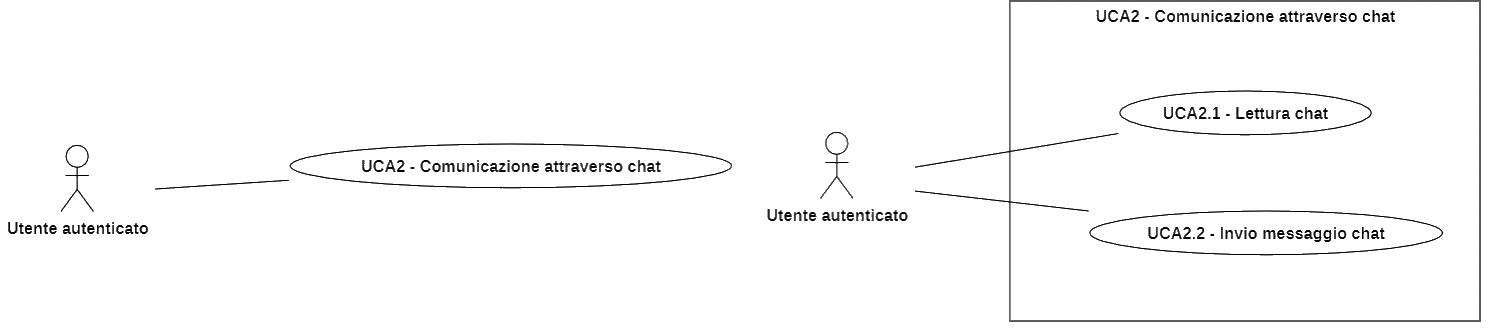
\includegraphics[width=0.999\textwidth]{./uml/UCA2.png} 
	\caption{Comunicazione attraverso \textit{chat}}
	\label{fig:UCA2}
  \end{figure}

\begin{itemize}
	\item \textbf{Attore principale:} Utente autenticato.

	\item \textbf{Precondizione:} L'Utente autenticato ha effettuato l'accesso al Sistema (vedi \autoref{usecase:Effettua accesso}).

	\item \textbf{Postcondizione:} La \textit{chat} è stata avviata.

	\item \textbf{Scenario principale:}
	      \begin{enumerate}
		      \item L'Utente base oppure ristoratore inizia la \textit{chat} con l'invio di un messaggio (vedi \autoref{usecase:Invio messaggio chat});
		            \begin{itemize}
			            \item L'Utente ristoratore può iniziare la \textit{chat} con l'invio di un messaggio ad un Utente base soltanto se ha effettuato una prenotazione (ved \autoref{usecase:Prenotazione di un tavolo}).
		            \end{itemize}
		      \item La \textit{chat} viene creata e inizializzata;
		      \item L'Utente base oppure ristoratore possono leggere i messaggi presenti in \textit{chat} (vedi \autoref{usecase:Lettura chat});
		      \item Ora l'Utente base e l'Utente ristoratore possono comunicare tra di loro attraverso l'uso della \textit{chat}, inviando e leggendo i messaggi vicendevolmente.
	      \end{enumerate}
\end{itemize}

\subusecaseautenticato{Lettura \textit{chat}}
\label{usecase:Lettura chat}
\begin{itemize}
	\item \textbf{Attore principale:} Utente autenticato.

	\item \textbf{Precondizione:} La \textit{chat} è stata avviata.

	\item \textbf{Postcondizione:} L'utente legge la \textit{chat} aggiornata.

	\item \textbf{Scenario principale:}
	      \begin{enumerate}
		      \item Il Sistema aggiorna la \textit{chat} all'ultimo messaggio inviato;
		      \item L'utente legge l'ultimo messaggio che gli è stato inviato.
	      \end{enumerate}
\end{itemize}


\subusecaseautenticato{Invio messaggio \textit{chat}}
\label{usecase:Invio messaggio chat}
\begin{itemize}
	\item \textbf{Attore principale:} Utente autenticato.

	\item \textbf{Precondizione:} La \textit{chat} è stata avviata.


	\item \textbf{Postcondizione:} Il messaggio scritto è stato inviato in \textit{chat}.

	\item \textbf{Scenario principale:}
	      \begin{enumerate}
		      \item L'Utente autenticato scrive ed invia un messaggio in \textit{chat};
		      \item Il Sistema memorizza il messaggio.
	      \end{enumerate}
\end{itemize}
